% =====================================================================
% CAEM — Supervisor presentation
% Compile:  pdflatex caem_supervisor.tex  (twice for refs)
% Author:   Aksan Gony Alif (BRAC CSE400)
% =====================================================================
\documentclass[10pt,aspectratio=169]{beamer}
\usetheme{Boadilla}
\usecolortheme{seahorse}
\useinnertheme{rectangles}
\useoutertheme{infolines}
\setbeamertemplate{navigation symbols}{}

\usepackage{amsmath,amssymb,booktabs,array}
\usepackage[T1]{fontenc}
\usepackage{tikz}
\usetikzlibrary{arrows.meta,positioning,fit,shapes.geometric,calc}
\usepackage{xcolor}

\definecolor{caemblue}{RGB}{31,82,142}
\definecolor{caemamber}{RGB}{200,140,30}
\definecolor{caemgreen}{RGB}{50,120,60}

\setbeamercolor{block title}{bg=caemblue,fg=white}
\setbeamercolor{block body}{bg=caemblue!8,fg=black}

\title[CAEM]{Confidence-Aware Episodic Memory with Self-Improvement}
\subtitle{An architectural intervention for hallucination reduction}
\author{Aksan Gony Alif}
\institute[BRAC University]{BRAC University \\ CSE400 Senior Thesis}
\date{\today}

% ---- Helpers ----------------------------------------------------------
\newcommand{\code}[1]{{\small\texttt{#1}}}

\begin{document}

% =====================================================================
\begin{frame}
  \titlepage
\end{frame}

% =====================================================================
\begin{frame}{The problem}
  \begin{itemize}
    \item Large language models hallucinate at \textbf{3\%--91\%} across deployment domains \\
          (Alkaissi 2023; Huang et al.\ ACM 2024).
    \item TruthfulQA shows hallucination is \textbf{not solved by scale}: bigger models often hallucinate \emph{more} confidently (Lin et al.\ 2022).
    \item Existing fixes are \emph{post-hoc detectors} added to a fixed model: they label outputs but cannot \emph{change} what the system serves.
  \end{itemize}

  \vspace{0.6em}
  \begin{block}{Thesis claim}
    Treat hallucination reduction as a \textbf{system-level architectural} problem, not a detection problem.
    Pair the model with an \emph{episodic memory}, a \emph{calibrated verifier ensemble}, a \emph{conformal storage gate}, and a \emph{cycle-boundary update loop} that improves the model from its own verified outputs.
  \end{block}
\end{frame}

% =====================================================================
\begin{frame}{CAEM at a glance}
  \begin{columns}[t]
    \column{0.55\textwidth}
    \textbf{Per-query path (8 stages, $\sim$10\,s):}
    \begin{enumerate}\setlength\itemsep{0.1em}\small
      \item Pre-routing confidence $u_{\text{pre}}$
      \item Encode + memory lookup
      \item Three-tier router (with safety override)
      \item Tier execution (memory / zero-shot / RAG)
      \item Nine-signal verifier ensemble
      \item Calibrated composite + conformal gate
      \item Output (STORE / DEFER / ABSTAIN / DISCARD)
      \item Per-query housekeeping
    \end{enumerate}

    \column{0.45\textwidth}
    \textbf{Per-cycle update (every 9000 queries):}
    \begin{itemize}\setlength\itemsep{0.1em}\small
      \item SIL fine-tune w/ L2 anchor + retention guard
      \item Cal-fold scoring under post-SIL model
      \item Re-fit $T$, isotonic curves, conformal $\tau$
      \item Reload verifier
      \item Retroactive re-verify all stored entries
      \item Stream chunk + eval-fold
    \end{itemize}
  \end{columns}

  \vspace{0.5em}
  {\small Backbone: Qwen-2.5-3B-Instruct. Verifier judge: MiniCheck (Flan-T5-Large). Encoder: SBERT all-mpnet-base-v2. Retrieval: 21M-passage DPR over Wikipedia.}
\end{frame}

% =====================================================================
\begin{frame}{Pipeline diagram (single query)}
  \centering
  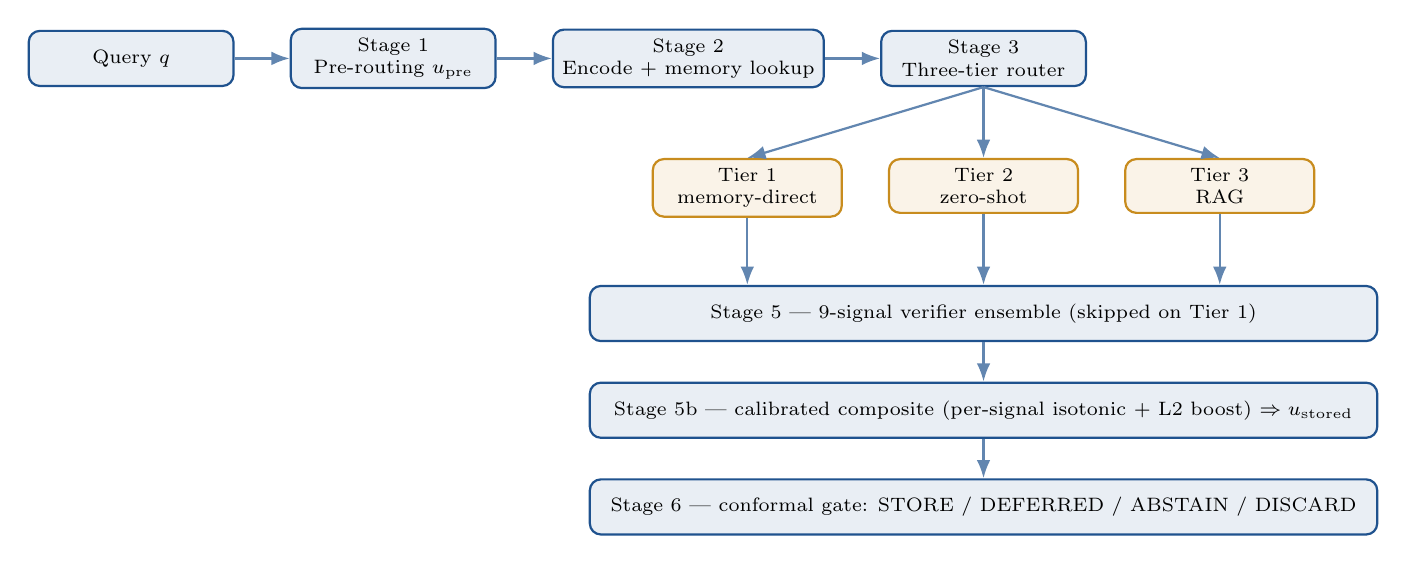
\begin{tikzpicture}[
      node distance=0.55cm and 0.7cm,
      stage/.style={draw=caemblue,thick,fill=caemblue!10,rounded corners,
                    minimum width=2.6cm,minimum height=0.7cm,align=center,font=\scriptsize},
      tier/.style={draw=caemamber,thick,fill=caemamber!10,rounded corners,
                   minimum width=2.4cm,minimum height=0.6cm,align=center,font=\scriptsize},
      arrow/.style={-Latex,thick,caemblue!70}
  ]
    \node[stage] (q) {Query $q$};
    \node[stage,right=of q]    (s1) {Stage 1\\ Pre-routing $u_{\text{pre}}$};
    \node[stage,right=of s1]   (s2) {Stage 2\\ Encode + memory lookup};
    \node[stage,right=of s2]   (s3) {Stage 3\\ Three-tier router};

    \node[tier,below=0.9cm of s3,xshift=-3cm] (t1) {Tier 1\\ memory-direct};
    \node[tier,below=0.9cm of s3]              (t2) {Tier 2\\ zero-shot};
    \node[tier,below=0.9cm of s3,xshift=3cm]  (t3) {Tier 3\\ RAG};

    \node[stage,below=0.9cm of t2,minimum width=10cm] (s5) {Stage 5 — 9-signal verifier ensemble (skipped on Tier 1)};
    \node[stage,below=0.5cm of s5,minimum width=10cm] (s5b) {Stage 5b — calibrated composite (per-signal isotonic + L2 boost) $\Rightarrow u_{\text{stored}}$};
    \node[stage,below=0.5cm of s5b,minimum width=10cm] (s6) {Stage 6 — conformal gate: STORE / DEFERRED / ABSTAIN / DISCARD};

    \draw[arrow] (q) -- (s1);
    \draw[arrow] (s1) -- (s2);
    \draw[arrow] (s2) -- (s3);
    \draw[arrow] (s3.south) -- (t1.north);
    \draw[arrow] (s3.south) -- (t2.north);
    \draw[arrow] (s3.south) -- (t3.north);
    \draw[arrow] (t1.south) -- (s5.north -| t1.south);
    \draw[arrow] (t2.south) -- (s5.north);
    \draw[arrow] (t3.south) -- (s5.north -| t3.south);
    \draw[arrow] (s5) -- (s5b);
    \draw[arrow] (s5b) -- (s6);
  \end{tikzpicture}
\end{frame}

% =====================================================================
\begin{frame}{Stage 1 — Pre-routing confidence $u_{\text{pre}}$}
  \textbf{Goal:} a single calibrated scalar saying ``model is ready'' or ``model is unsure'', \emph{before} we commit any expensive compute.

  \vspace{0.5em}
  \textbf{Two cheap signals from one short forward pass:}
  \begin{itemize}\small
    \item $u_{\text{token}}$ — geometric mean of per-token log-probabilities of the draft answer.
    \item $c_{\text{conv}}$ — encoder-layer convergence ratio (variance of early layers / variance of late layers; high $=$ unstable).
  \end{itemize}

  \vspace{0.5em}
  \textbf{Fused with fixed weights, then temperature-scaled:}
  \[
    u_{\text{pre}} \;=\; \sigma\!\left(\frac{\operatorname{logit}\bigl(0.60\,u_{\text{token}} + 0.40\,(1{+}c_{\text{conv}})^{-1}\bigr)}{T}\right).
  \]
  $T$ is re-fit at every cycle boundary by ECE minimisation on a 1500-sample held-out fold.

  \vspace{0.5em}
  \begin{block}{Why this matters}
    $u_{\text{pre}}$ is the gate that lets the router \emph{refuse} the cheap memory or zero-shot tier when the model is unsure. The safety floor at $u_{\text{pre}} \ge 0.60$ is the OR-condition that puts model readiness on equal footing with memory quality.
  \end{block}
\end{frame}

% =====================================================================
\begin{frame}{Stages 2--3 — Memory and the three-tier router}
  \textbf{Memory:} FAISS index over SBERT embeddings of past verified $(q, a)$ pairs. Top-1 search returns similarity $s$ and the neighbour's stored quality $u_{\text{stored}}$.

  \vspace{0.4em}
  \textbf{Combined dispatch score:}
  \[
    \mathcal{S} \;=\; \lambda \cdot s \;+\; (1-\lambda)\cdot u_{\text{stored}} \quad\text{with}\ \lambda = 0.70.
  \]

  \vspace{0.4em}
  \textbf{Decision rules (in fixed order):}
  \begin{enumerate}\small
    \item \textbf{Safety override:} if $u_{\text{pre}} < 0.60 \Rightarrow$ \textbf{Tier 3} regardless of $\mathcal{S}$.
    \item \textbf{Tier 1} (memory-direct) if $\mathcal{S} \ge 0.90$ — serve the neighbour, no generation.
    \item \textbf{Tier 2} (zero-shot) if similarity $> 0.75$ — generate without retrieval.
    \item \textbf{Tier 3} (RAG) — retrieve from 21M-passage corpus, rerank, generate grounded.
  \end{enumerate}

  \vspace{0.4em}
  \begin{block}{Cost--quality property}
    Tier 1 amortises away the verifier as the memory grows; Tier 3 is the architectural floor when nothing else has earned the right. Tier-1 share grows with cycle index $\Rightarrow$ memory-direct serving compounds cost savings.
  \end{block}
\end{frame}

% =====================================================================
\begin{frame}{Stage 5 — Nine-signal verifier ensemble (four families)}
  \footnotesize
  \begin{tabular}{@{}p{2.6cm}p{4cm}p{6cm}@{}}
    \toprule
    \textbf{Family} & \textbf{Signal} & \textbf{Reads what failure mode} \\
    \midrule
    Internal calibration & $u_{\text{token}}$ & Token-level confidence (cheap) \\
                         & $u_{\text{dropout}}$ & MC-Dropout variance, $K{=}5$ passes \\
                         & $u_{\text{internal}} = \tfrac{1}{2}u_{\text{token}}{+}\tfrac{1}{2}(1{-}u_{\text{dropout}})$ & Combined internal stability \\
    \midrule
    Sample-set agreement & $s_{\text{avg}}$ & Cosine similarity over $M{=}3$ resampled chains \\
                         & $p_{\text{entail}}$ & NLI entailment chain $\to$ served answer \\
    \midrule
    External grounding   & $p_{\text{ground,max}}$ & Top-1 retrieved-passage entailment \\
                         & $p_{\text{ground,mean}}$ & Mean over top-3 \\
                         & $p_{\text{ground,atomic}}$ & Length-gated atomic-fact decomp \\
    \midrule
    Q-A relevance        & $q_{\text{a,rel}}$ & Independent cross-encoder, question vs.\ answer \\
    \bottomrule
  \end{tabular}

  \vspace{0.4em}
  \begin{block}{Empirical retirement of $h_{\text{norm}}$}
    The 10th candidate (normalised semantic entropy, $K{=}10$) was retired post Cycle-0 audit: fitted boost weight $-5\times10^{-4}$, statistically zero. Cost was $\sim$4\,s/sample. Replaced by a constant sentinel; locked artefacts preserved.
  \end{block}
\end{frame}

% =====================================================================
\begin{frame}{Stage 5b — Calibrated probability composite}
  \textbf{Aggregation pipeline:}
  \begin{enumerate}\small
    \item Per-signal \textbf{isotonic regression} $P_j = \mathrm{iso}_j(\mathrm{signal}_j)$ on the cycle-0 cal-fold.
    \item Convert to log-odds $L_j = \log\bigl(P_j/(1-P_j)\bigr)$.
    \item \textbf{L2-regularised logistic boost} (Cherian 2024): $\operatorname{logit}(u_{\text{stored}}) = b + \sum_j w_j L_j$ with $C = 0.01$.
    \item Sigmoid back: $u_{\text{stored}} = \sigma(\cdot) \in (0,1)$.
  \end{enumerate}

  \vspace{0.5em}
  \textbf{Locked Cycle-0 weights (most informative):}
  \begin{tabular}{@{}lr|lr@{}}
    $q_{\text{a,rel}}$ & $\mathbf{+0.500}$ & $u_{\text{token}}$ & $+0.188$ \\
    $p_{\text{ground,mean}}$ & $+0.290$ & $p_{\text{ground,max}}$ & $+0.164$ \\
    $p_{\text{ground,atomic}}$ & $+0.290$ & $s_{\text{avg}}$ & $+0.101$ \\
    $u_{\text{internal}}$ & $+0.204$ & $p_{\text{entail}}$ & $+0.094$ \\
    \multicolumn{4}{@{}c@{}}{intercept $b = +1.099$, em\_rate on cal-fold $= 0.243$} \\
  \end{tabular}

  \vspace{0.4em}
  Grounding family carries 0.74 of the weight; $q_{\text{a,rel}}$ alone carries 0.50. Internal signals are useful but secondary.
\end{frame}

% =====================================================================
\begin{frame}{Stage 6 — Conformal storage gate (the four outcomes)}
  \textbf{Split-CP with two miscoverage targets:}
  \begin{itemize}\small
    \item $\alpha_{\text{store}} = 0.05 \Rightarrow$ precision target 0.95 \quad $\to \tau_{\text{store}} = 0.6676$
    \item $\alpha_{\text{defer}} = 0.40 \Rightarrow$ precision target 0.60 \quad $\to \tau_{\text{defer}} = 0.5207$
  \end{itemize}

  \vspace{0.4em}
  \textbf{Decision rule:}
  \[
  \texttt{decision}=\begin{cases}
    \texttt{STORE}    & u_{\text{stored}} \ge \tau_{\text{store}} \\
    \texttt{DEFERRED} & \tau_{\text{defer}} \le u_{\text{stored}} < \tau_{\text{store}} \\
    \texttt{ABSTAIN}  & u_{\text{stored}} < \tau_{\text{defer}} \text{ AND } p_{\text{ground,max}} < 0.20 \\
    \texttt{DISCARD}  & \text{otherwise}
  \end{cases}
  \]

  \vspace{0.3em}
  \textbf{Confabulation early-exit (precedence over composite):}
  \[
  u_{\text{internal}} \ge 0.70 \;\wedge\; p_{\text{ground,max}} \le 0.20 \;\Rightarrow\; \texttt{DISCARD},\ \text{escalate to Tier 3}.
  \]
  Catches the dangerous corner: ``model is sure but evidence directly contradicts.''

  \vspace{0.3em}
  \begin{block}{Per-query precision contract (theorem 1)}
    Under exchangeability, empirical precision on the STORE class is bounded below by $1 - \alpha_{\text{store}} = 0.95$. Plain fine-tuning structurally cannot produce this guarantee.
  \end{block}
\end{frame}

% =====================================================================
\begin{frame}{Stage 8 — Cycle-boundary update loop}
  \footnotesize
  \begin{enumerate}
    \item \textbf{SIL fine-tune.} CE loss on 137 verified episodes + 15 general items. L2 anchor $\lambda_{\text{anc}}\|\theta - \theta_{t-1}\|^2$ (first-order EWC). 3 epochs at effective batch 16. \textbf{Retention guard:} if MMLU drops below $\rho_{\min}{=}0.93$ of pristine, abort cycle, restore $\theta_{t-1}$, \emph{keep memory}.
    \item \textbf{Step 2.1.} Score the same 1500-sample cal-fold under the post-SIL model; cache $u_{\text{pre}}$ + 9 signals + EM per sample.
    \item \textbf{Step 2.2.} Re-fit $T$ by ECE minimisation. Reads $u_{\text{pre}}$ from the cache (recently optimised — saves $\sim$3.5\,h/cycle).
    \item \textbf{Step 2.3.} Re-fit per-signal isotonic curves and conformal $\tau$ on the post-SIL fold. EMA-smooth: $\tau_{\text{new}} = 0.7\,\tau_{\text{prev}} + 0.3\,\tau_{\text{fit}}$.
    \item \textbf{Step 2.4.} Hot-swap the verifier with the cycle-$N$ JSONs.
    \item \textbf{Step 2.5.} Retroactive re-verification: re-score every stored entry; prune below $\tau_{\text{retro}} = 0.50$, otherwise upgrade upward (monotone).
    \item \textbf{Step 4.} Cycle-$N$ stream chunk: 9000 new queries through the full pipeline, populate memory.
    \item \textbf{Step 5.} Cycle-$N$ eval-fold: 3500 samples (500 $\times$ 7 benchmarks) for headline EM/F1/CHM.
  \end{enumerate}
\end{frame}

% =====================================================================
\begin{frame}{Worked example — one TriviaQA query}
  \footnotesize
  \textbf{Question:} \emph{Who duetted with Aretha Franklin on ``Sisters Are Doin' It for Themselves''?}

  \textbf{Model's draft:} ``Annie Lennox'' \quad (gold answer: \emph{Annie Lennox} — \textbf{correct})

  \vspace{0.4em}
  \begin{tabular}{@{}lr|lr@{}}
    $u_{\text{token}}$       & 0.059 & $p_{\text{entail}}$        & 0.059 \\
    $u_{\text{dropout}}$     & 0.80  & $p_{\text{ground,max}}$    & 0.040 \\
    $u_{\text{internal}}$    & 0.130 & $p_{\text{ground,mean}}$   & 0.038 \\
    $s_{\text{avg}}$         & 0.939 & $p_{\text{ground,atomic}}$ & 0.038 \\
    \multicolumn{2}{@{}l|}{$q_{\text{a,rel}} = 0.507$} & \multicolumn{2}{@{}l@{}}{$\Rightarrow u_{\text{stored}} = 0.239$} \\
  \end{tabular}

  \vspace{0.4em}
  $u_{\text{stored}} < \tau_{\text{defer}} = 0.521$ \emph{and} $p_{\text{ground,max}} < 0.20 \Rightarrow$ \textbf{ABSTAIN}.

  \vspace{0.5em}
  \begin{block}{What the system actually serves}
    User receives ``\emph{I do not know.}'' with confidence label \emph{very low}.
    \\
    \textbf{Why:} the answer is right but \emph{the evidence trail is empty} — token-level uncertainty, MC-Dropout instability, no passage entailment. From the verifier's perspective, the same signal profile applies to any plausible-sounding hallucination. The architecture protects the precision contract by abstaining; one correct rare-fact answer is rejected so that the storage pool stays at $\ge 95\%$ purity.
  \end{block}
\end{frame}

% =====================================================================
\begin{frame}{Why CAEM beats plain exact-match-labelled fine-tuning}
  \emph{At the same labelling budget, the simpler baseline is plain fine-tuning. CAEM's load-bearing wins:}

  \begin{enumerate}\small
    \item \textbf{Per-query precision contract} — conformal-bounded $1{-}\alpha_{\text{store}} = 0.95$ at every served STORE; fine-tuning cannot produce this.
    \item \textbf{Memory-direct serving tier} — Tier-1 hit-rate compounds cost savings as the verified pool grows; fine-tuning still pays a full forward pass per query.
    \item \textbf{Asymmetric rollback} — a failed cycle restores weights but \emph{keeps memory}; fine-tuning's ``failed run'' loses everything.
    \item \textbf{Verifier as sample-efficiency multiplier} — the cycle-boundary labelled batch validates a precision contract; the gradient signal does not have to carry it directly.
    \item \textbf{Inference-time error catching} — verifier keeps running after the fine-tune saturates against the model's parametric capacity ceiling. Fine-tuning has nowhere left to go once that ceiling is hit.
  \end{enumerate}
\end{frame}

% =====================================================================
\begin{frame}{Theoretical guarantees (paired with empirical receipts)}
  \footnotesize
  \begin{enumerate}
    \item \textbf{Pool purity floor.} Under upward-only retroactive update, $\pi_t \ge 1 - \alpha_{\text{store}}$ for all $t$. \\
          \emph{Receipt:} per-cycle pool purity should not drop below $\min(0.95, \pi_{\text{retro}})$.
    \item \textbf{Monotonicity in verifier discrimination.} Storage rate and pool purity both rise with the cal-fold Cohen's $d$. \\
          \emph{Receipt:} $d_t$ vs $\sigma_t$ trajectory across cycles in Ch5.
    \item \textbf{Geometric envelope.} $|\pi_t - \pi_\infty| = \mathcal{O}(r^t)$ with contraction rate $r = \mathcal{O}\!\bigl(\sigma\,\Phi(d/\sqrt{2})\bigr)$. \\
          \emph{Receipt:} exponential-decay fit to $G_t = |\pi_t - \pi_\infty|$ across cycles.
    \item \textbf{Asymptotic Tier-1 hallucination floor.} $H_\infty \le \alpha_{\text{store}} + (1{-}\alpha_{\text{store}})\,\varepsilon_{\text{arch}}$. \\
          The hallucination floor is set by \emph{conformal level}, not by deployment scale.
  \end{enumerate}
\end{frame}

% =====================================================================
\begin{frame}{Locked Cycle-0 configuration (on disk before main run)}
  \small
  \begin{tabular}{@{}lr@{\quad}lr@{}}
    \toprule
    \textbf{Quantity} & \textbf{Value} & \textbf{Quantity} & \textbf{Value} \\
    \midrule
    $\tau_{\text{store}}$ & 0.6676 & boost intercept $b$ & $+1.099$ \\
    $\tau_{\text{defer}}$ & 0.5207 & boost L2 $C$ & 0.01 \\
    $\alpha_{\text{store}}$ & 0.05 & $n_{\text{store}}$ on cal-fold & 56 \\
    $\alpha_{\text{defer}}$ & 0.40 & $\pi_{\text{store}}$ (cal-fold) & 0.9643 \\
    $\alpha_{\text{ema}}$ & 0.7 & $\pi_{\text{defer}}$ (cal-fold) & 0.6021 \\
    $\rho_{\min}$ retention & 0.93 & em\_rate (cal-fold) & 0.243 \\
    $\tau_{\text{retro}}$ prune & 0.50 & cal-fold size & 1500 \\
    safety floor $u_{\text{pre}}^{\min}$ & 0.60 & cycles in main run & 10 \\
    Tier-1 threshold & 0.90 & queries/cycle (training) & 9000 \\
    Tier-2 sim threshold & 0.75 & eval-fold (held-out) & 3500 \\
    \bottomrule
  \end{tabular}

  \vspace{0.5em}
  All thresholds, fits, and validations were committed to git \emph{before} the empirical record was consulted (pre-registration discipline). Receipts in \code{outputs/cycle\_0/\{composite\_calibration, conformal\_gate\}.json}.
\end{frame}

% =====================================================================
\begin{frame}{Empirical campaign — current status}
  \small
  \begin{itemize}
    \item \textbf{Cycle 0:} done. Locked configuration drawn from a 25-variant pre-registered sweep over $(\alpha_{\text{store}}, C)$, selected $\alpha = 0.05$, $C = 0.01$.
    \item \textbf{Cycle 1:} running today. SIL fine-tune complete (loss 1.276 $\to$ 0.722, MMLU retention 1.0000). Step 2.1 cal-fold scoring in progress.
    \item \textbf{Step 7 main:} 10-cycle SIL trajectory under way. ETA $\sim$5.5 days under current optimisations.
    \item \textbf{Phase 4 (after main):} external baselines B1--B7 on matched protocol, paired McNemar + BCa bootstrap under Holm correction, purity validation, Ch5 table generation.
  \end{itemize}

  \vspace{0.4em}
  \textbf{Live optimisations applied this week:}
  \begin{itemize}\small
    \item Empirical retirement of $h_{\text{norm}}$ (boost weight $\approx 0$) — saved $\sim$50\,h over the trajectory.
    \item $u_{\text{pre}}$ cache fast-path on Step 2.2 — saves $\sim$3.5\,h per cycle.
    \item OOM mitigation suite ($\theta_{t-1}$ on CPU, force-eager compile, batch 4 $\times$ grad-accum 4, expandable allocator) for the 32 GB 5090 envelope.
  \end{itemize}
\end{frame}

% =====================================================================
\begin{frame}{Contribution summary}
  \begin{block}{Architectural contribution}
    An eight-stage pipeline that combines an episodic memory, a confidence-aware three-tier router, a nine-signal verifier ensemble, a calibrated-probability composite, and a conformal split-CP storage gate, wrapped in a cycle-boundary self-improvement loop with retention guard.
  \end{block}

  \begin{block}{Theoretical contribution}
    Four theorems characterise the storage-class trajectory: pool-purity floor, monotonicity in verifier discrimination, geometric envelope, and asymptotic hallucination floor set by the conformal level rather than by scale.
  \end{block}

  \begin{block}{Engineering contribution}
    A reproducible pre-registered empirical pipeline: every threshold, fit-time procedure, and artefact path committed to code \emph{before} the empirical record is consulted; every architectural decision paired with a verifiable on-disk receipt.
  \end{block}
\end{frame}

% =====================================================================
\begin{frame}
  \centering
  \vspace{1.5cm}
  {\Huge\textbf{Thank you.}}\\[0.8em]
  {\large Questions?}\\[1.5em]
  {\small Aksan Gony Alif \quad $\cdot$ \quad BRAC University CSE400 \quad $\cdot$ \quad \today}
\end{frame}

\end{document}
